\documentclass{standalone}
\usepackage{amssymb,amsmath}
\usepackage{tikz}
\usetikzlibrary{automata,positioning,matrix,shapes.callouts}
\begin{document}
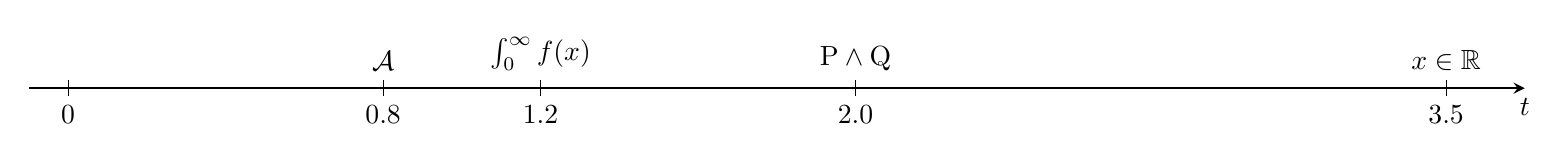
\begin{tikzpicture}
% scale
\draw [thick, -stealth](-0.5,0)--(18.500000,0) node [anchor=north]{$t$};
\draw (0,0.1) -- (0,-0.1) node [anchor=north]{$0$};

% alphabets
\draw (4.000000,0.1) node[anchor=south]{$\mathcal{A}$} -- (4.000000,-0.1) node[anchor=north]{0.8};
\draw (6.000000,0.1) node[anchor=south]{$\int_0^\infty f(x)$} -- (6.000000,-0.1) node[anchor=north]{1.2};
\draw (10.000000,0.1) node[anchor=south]{$\mathrm{P} \land \mathrm{Q}$} -- (10.000000,-0.1) node[anchor=north]{2.0};
\draw (17.500000,0.1) node[anchor=south]{$x \in \mathbb{R}$} -- (17.500000,-0.1) node[anchor=north]{3.5};
\end{tikzpicture}
\end{document}
